\chapter{ Architektura systemu: przegląd i wybór technologii } \label{chapter_architecture}

\section{Zarys architektury}

\begin{figure}[H]
\centering\small
\caption{
	Zarys architektury systemu
}
\label{top_level_architecture_diagram}
\hspace{-1.2cm}
\begin{forest}
	% forest preamble: determine layout and format of tree
	direction switch,
	for tree={fork sep=3em}
	[ System inspekcji obszarów,yshift=3em,alias=LP
	  [ \textbf{Dron}
		[ Kontroler lotu ]
		[ Komputer pokładowy
		 [ Wyznaczanie trasy lotu ]
		 [ Wysyłanie telemetrii ]
		 [ Wysyłanie zdjęć ]
		]
		[ Kamera ]
		[ Modem GSM ]
	  ]
	  [ \textbf{Serwer webowy}, yshift=0.5cm
		[ Obsługa telemetrii
			[ Odbiór danych z drona ]
			[ Przekazywanie do klientów ]
			[ Przygotowanie do archiwizacji ]
		]
		[ Rest API: odczyt i zapis
		  [ Logów telemetrii ]
		  [ Tras lotów ] 
		  [ Harmonogramu lotów ]
		  [ Raportów z lotów ]
		]
		[ Sztuczna inteligencja
		  [ Analiza obrazów z lotów ]
		]
	  ]
	  [ \textbf{Aplikacja kliencka}, xshift=0.1cm
		[ Planowanie 
			[ Tras lotów ]
			[ Harmonogramu lotów ]
		]
		[ Odbiór telemetrii ]
		[ Przegląd raportów z lotów 
		  [ Trasa lotu ]
		  [ Rozpoznane na zdjęciach obiekty ]
		]
	  ]
	]
%   \draw[thick]
%   ([yshift=-1.5em]LP.south)  -- ++(-6em,0) node[left,draw,font=\sffamily,thin]{ABC}
%   ([yshift=-1.5em]LP.south)  -- ++(6em,0) node[right,draw,font=\sffamily,thin]{XYZ};
  \end{forest}
\end{figure}

% \begin{tikzpicture}
	
% 	\node[entity](backend) {Serwer webowy}
% 	[];
% 	\node[entity](backend_telem) {Podsystem obsługujący telemetrię}[
% 		below right = of backend
% 	];

% 	% \node[entity] (dron) {Dron}
% 	%   [grow=up,sibling distance=3cm];
	
	
	 
% \end{tikzpicture}

\section{Dron}

\subsection{Kontroler lotu}

Wielowirnikowce podłączone do systemu, muszą być
wyposażone w kontroler lotu -- umożliwiający
autonomiczny lot, stabilizację oraz obsługę 
peryferiów takich jak czujniki oraz silniki.

Spośród aktywnie rozwijanych i popularnych
projektów \cite{autopilots_sourvey} tworzących oprogramowanie do kontrolerów
lotu, można wyróżnić cztery najpopularniejsze inicjatywy: 

\begin{table}[htb]
	\centering\small
	\caption{
		Najpopularniejsze otwarte projekty
		oprogramowania obsługującego kontrolery lotu
	}
	\label{flight_controllers_comparison}

	\begin{tabularx}{0.87\textwidth}
	{ 
	| >{\raggedright\arraybackslash}l 
	| c 
	| >{\raggedright\arraybackslash}X
	| >{\raggedleft\arraybackslash}l |
	}
	\hline
	\textbf{Nazwa projektu} & \textbf{Rok założenia} &
	\textbf{Docelowy hardware}
	&  \textbf{Licencja}
	\\\hline
	ArduPilot\cite{ardupilot_home_page}		&  2009	& otwarte mikrokontrolery ARM & GPLv3
	\\ \hline
	AutoQuad\cite{autoquad_timeline}		&  2011	& mikrokontrolery STM Cortex M4		 & GPLv3
	\\ \hline
	LibrePilot\cite{librepilot_home_page}	&  2015	& zamknięte źródłowo kontrolery lotu, bazujące na architekturze ARM & GPLv3
	\\ \hline       
	PX4 Autopilot\cite{px4_home_page}		&  2012	& otwarte mikrokontrolery ARM & BSD
	\\ \hline       
	\end{tabularx}
	
\end{table}

Spośród wymienionych projektów, ArduPilot posiada najbardziej rozbudowaną bazę 
dokumentacji i instrukcji. Architektura projektu umożliwia skompilowanie projektu
na standardowy komputer typu PC uruchomienie go w wirtualnym
środowisku\cite{ardupilot_sitl}, co ułatwia proces testowania oprogramowania,
które steruje dronem -- model maszyny jest symulowany, jednak warstwa komunikacji
jest dokładnie taka sama, jak w przypadku pracy z prawdziwym dronem. Dodatkowo, projekt
realizowany był w kole studenckim, w którym ArduPilot jest od lat wykorzystywany
do sterowania dronami i samolotami, co przesądziło o zastosowaniu go jako
oprogramowanie do kontrolera lotu.

\subsection{Komputer pokładowy}

Poza kontrolerem lotu, który zawiera jedynie oprogramowanie 
niezbędnie do sterowania dronem i udostępniania
strumienia telemetriii, na maszynie musi znaleźć się też komputer pokładowy, 
do zastosowań bardziej ogólnych. Będzie on wykorzystywany do
obsługi wysokopoziomowych peryferiów: kamery oraz modemu GSM. Do zadań
komputera pokładowego będzie należała także realizacja logiki biznesowej systemu
- odczytanie harmonogramu przelotów z serwera webowego i załadowanie do kontrolera lotu
konkretnej trasy przelotu.

\subsubsection{Wymagania sprzętowe}

Aby wypełniać zadania wymienione powyżej, komputer pokładowy musi
posiadać następujące interfejsy sprzętowe:

\begin{itemize}
	\item \texttt{UART} -- do komunikacji z kontrolerem lotu,
	\item \texttt{USB} -- do komunikacji z modemem,
	\item \texttt{CSI} -- do komunikacji z kamerą.
\end{itemize}

Większość dostępnych na rynku komputerów klasy SBC (\textit{Single-board Computer})
posiada powyższe interfejsy, więc wymagania sprzętowe nie są tutaj ograniczeniem.
W projekcie został wykorzystany najpopularniejszy do zastosowań amatorskich
komputer \textit{Raspberry Pi}. 

\subsubsection{Oprogramowanie}

Na komputerze pokładowym zainstalowany jest system Linux -- gwarantuje to bezproblemową
obsługę peryferiów oraz dostępność stosu sieciowego, koniecznego do przesyłania 
danych telemetrycznych i zdjęć.
Dodatkowo, wymagane jest oprogramowanie dekodujące
i enkodujące wiadomości protokołu \textit{MavLink}, który jest wykorzystywany przez 
ArduPilota do komunikacji z zewnętrznymi systemami \cite{ardupilot_mavlink}.

Infrastruktura projektu ArduPilot dostarcza gotowe narzędziae do
parsowania i tworzenia wiadomości w protokole \textit{MavLink}.
Jedną z nich jest \texttt{pymavlink} - implementacja protokołu \textit{MavLink} 
w języku Python. \texttt{pymavlink} zawiera podstawowe funkcje i obiekty konieczne
do komunikacji z kontrolerem lotu. Biblioteka jest niskopoziomowa i nie w całości
napisana w sposób obiektowy -- finalnie wykorzystujemy więc bibliotekę
\texttt{dronekit-python}\cite{dronekit_python}, która rozbudowuje \texttt{pymavlink}
o w pełni obiektowy, wysokopoziomowy interfejs do komunikacji z kontrolerem lotu. 
Skrypty odpowiedzialne za logikę biznesową napisane są w Pythonie.

\section{Protokoły wymiany danych}

\subsection{Dane telemetryczne - biblioteka \texttt{protobuf}} \label{protobuf_chapter}

% W trakcie lotu, drony regularnie wysyłają dane telemetryczne -- 
% informują o swoim obecnym położeniu, podają stan baterii oraz .

W trakcie lotu, drony regularnie wysyłają dane telemetryczne. Każdy pakiet
danych telemetrycznych w systemie zawiera następujące informacje:
\begin{itemize}
	\item unikatowy identyfikator maszyny,
	\item identyfikator lotu (unikatowy dla każdej maszyny),
	\item pozycję odczytaną z odbiornika GPS,
	\item poziom naładowania baterii,
	\item informacja czy w obecnej chwili wykonywane są zdjęcia z lotu,
	\item timestamp w standardowym 32-bitowym formacie unixowym.
\end{itemize}

Nie jest wykluczone, że w przyszłości
może pojawić się potrzeba dołączenia do danych telemetrycznych nowych informacji,
na przykład w przypadku, gdy do maszyny zostanie dodane nowe oprzyrządowanie,
lub gdy system byłby adaptowany do obsługi innego rodzaju misji.
Dodatkowo, skala projektu wymusza utrzymywanie implementacji tego samego protokołu w wielu
różnych językach programowania -- oprogramowanie wysyłające telemetrię z drona napisane
jest w Pythonie, interfejs webowy wyświetlający telemetrię będzie musiał być jednak napisany
w języku JavaScript (ponieważ tylko ten język jest wspierany przez przeglądarki internetowe).
W~przyszłości może pojawić się konieczność dodania wsparcia dla innego języka programowania
-- na przykład gdyby do systemu miałby być dodany kolejny komponent. Jest to potencjalne
źródło problemów związanych z integracją między komponentami systemu, ponieważ wraz
z~dodawaniem kolejnych danych telemetrycznych i zwiększaniem liczby
wspieranych języków, rośnie szansa na popełnienie błędu w implementacji protokołu.
Nawet w przypadku dwóch równolegle wspieranych języków, utrzymywanie spójnej implementacji
protokołu nie jest zadaniem trywialnym -- szczególnie jeśli protokół wysyła dane
w formie binarnej, co jest konieczne, gdy jednym z wymagań jest wydajne zapakowanie danych. 

Jednym z możliwych rozwiązań tego problemu jest wykorzystanie narzędzi do generowania
kodu. Narzędzia tego typu pozwalają na zdefiniowanie standardu danych telemetrycznych
we własnym (specyficznym dla narzędzia) języku, opisującym strukturę danych przesyłanych
przez protokół. Następnie, narzędzia takie generują implementację protokołu w wybranych
językach programowania. Dzięki automatycznemu generowaniu implementacji protokołu,
programiści nie muszą dbać o spójność implementacji pomiędzy wieloma językami.

Wykorzystywanym w projekcie narzędziem do generowania implementacji protokołu jest
\texttt{protobuf} (\textit{Protocol Buffers})\cite{protocol_buffers} -- biblioteka
napisana w firmie Google, stworzona z myślą o zapewnianiu wydajnej komunikacji w czasie
rzeczywistym pomiędzy wieloma systemami informatycznymi. W obecnej wersji
(\texttt{v3.14.0}), biblioteka pozwala na generowanie kodu w językach:

\begin{multicols}{2}
\begin{itemize}
	\item Python
	\item C++
	\item Java
	\item C\#
	\item JavaScript
	\item Go
\end{itemize}
\end{multicols}

\begin{figure}[H]
	\centering\small
	\caption{
	 Diagram przedstawiający system generowania implementacji protokołu, na podstawie
	 narzędzia \texttt{protobuf}	
	}
	\label{protobuf_generation}
	\hspace{-1.2cm}
\tikzstyle{arrow} = [thick,->,>=stealth]
\begin{tikzpicture}[node distance=5cm]
	
	\node
		[entity](definitions)
		{ Definicje wiadomości };
	
	\node
		[trapezium, trapezium left angle=70, trapezium right angle=110, draw=black, right of = definitions, align=center](coompiler)
		{ Kompilator \texttt{protobuf} };
	
	\draw [arrow] (definitions) -- (coompiler);	
	
	% \node
	% 	[align=center, right of = coompiler, xshift=1.5cm](implementations)
	% 	{ Implementacje w wybranych \\ językach programowania };

	% \draw [arrow] (coompiler) -- (8.5, 0.4);	
	% \draw [arrow] (coompiler) -- (8.6, 0);	
	% \draw [arrow] (coompiler) -- (8.5, -0.4);
			
	\node
		[align = center, right of = coompiler, yshift=1.2cm, xshift=1.5cm](implementation_a)
		{Implementacja w języku A};
	\draw [arrow] (coompiler) -- (implementation_a.west);	
	
	\node
		[align = center, right of = coompiler, xshift=1.5cm](implementation_b)
		{Implementacja w języku B};
	\draw [arrow] (coompiler) -- (implementation_b);
	
	\node
		[align = center, right of = coompiler, yshift=-1.2cm, xshift=1.5cm](implementation_c)
		{Implementacja w języku C};	
	\draw [arrow] (coompiler) -- (implementation_c.west);

\end{tikzpicture}
\end{figure}

Poza automatycznym generowaniem
kodu protokołu, \texttt{protobuf} zapewnia także:

\begin{itemize}
	\item wydajne wykorzystanie miejsca -- biblioteka upakowuje dane w formie binarnej,
	\item kompatybilność wsteczną -- w przypadku dodania nowego typu pakietu telemetrii,
	implementacja zachowuje spójność z poprzednimi wersjami. Dzięki temu możliwe jest
	stopniowe wprowadzanie zmian w wielokomponentowym systemie,
	\item automatycznie generowane mechanizmy, pozwalające na sprawdzanie, czy dane 
	umieszczone w pakiecie telemetrii są poprawne (sprawdzanie typów, sprawdzanie
	czy zostały wypełnione wszystkie pola pakietu),
	\item interfejs programistyczny, umożliwiający samodzielne dopisanie wsparcia
	nowych języków do kompilatora \texttt{protobuf}.
\end{itemize}

\begin{lstlisting}[language=protobuf, label=list:protobuf,caption=Przykład definicji pakietu \texttt{protobuf}, basicstyle=\footnotesize\ttfamily]
syntax = "proto3";

package Telemetry;

/**
  Wiadomość zawierająca pozycję
  maszyny w trakcie lotu
*/
message Position {
  float lat = 1;
  float lng = 2;
  float alt = 3;
  float heading = 4;
}

message TelemFrameHeader {
  /* Flight metadata */
  int32 timestamp = 1;
  int32 machine_id = 2;
  int32 flight_id = 3;

  /**
	Kompozycja wcześniej
	zdefiniowanej wiadomości 
  */
  Position position = 4;
}
\end{lstlisting}

\begin{lstlisting}[language=Python, label=list:protobuf,caption=Przykład wykorzystania wygenerowanej implementacji pakietów w języku Python,basicstyle=\footnotesize\ttfamily]
# Wygenerowany moduł, zawierający definicje
# pakietów, domyślnie nosi nazwę definitions_pb2
import definitions_pb2
import time

header = definitions_pb2.TelemFrameHeader()

header.timestamp = int(time.time())
header.machine_id = 1
header.flight_id = 5

header.position.lat = 5
header.position.lng = 10
header.position.alt = 15
header.position.heading = 20

# Postać binarna, gotowa do zapisania do pliku
# lub wysłania przez protokół UDP/WebSocket
serialised_header = header.SerializeToString()
print("Serialised header:")
print(serialised_header) 
\end{lstlisting}

\subsection{Zdjęcia wysyłane w trakcie lotu - biblioteka \texttt{imagezmq}}

Wykonane przez drony zdjęcia wysyłane są na serwer webowyza pomocą biblioteki
\texttt{imagezmq}. Jak zaznaczono we wstępie, wysyłanie strumienia wideo to
temat zbyt skomplikowany, aby poruszać go w pracy -- rozwiązanie wykorzystywane
do przesyłu zdjęć zostało wybrane ze względu na prostotę instalacji i implementacji.

Biblioteka \texttt{imagezmq} pozwala wysyłać obrazy za pomocą protokołu \texttt{zmq}.
Przed wysłaniem, obrazy są kompresowane, jednak jest to kompresja ograniczająca się do 
pojedynczego kadru -- nie zaś strumienia obrazów, jak by to miało miejsce w przypadku 
strumieniowania filmu z lotu.

\section{Oprogramowanie serwerowe}

Serwer webowy jest punktem stykowym wszystkich elementów w systemie.
Na serwerze przechowywane są wszystkie dane konieczne do działania systemu, takie jak
trasy i harmonogramy lotów. Nadchodząca z dronów telemetria jest na 
serwerze multipleksowana i archiwizowana, pozwalając zarówno na odbieranie jej
w czasie rzeczywistym z poziomu aplikacji klienckiej, jak i na analizę już zakończonych lotów.

\subsection{Obsługa telemetrii}

System obsługujący dane telemetryczne odbiera nadchodzące z maszyn pakiety
\texttt{protobuf}, następnie w czasie rzeczywistym przekazuje je do aplikacji klienckich 
-- w ten sposób możliwy jest jednoczesny odbiór telemetrii na dowolnie wielu urządzeniach.
Poszczególne loty rozróżnialne są za pomocą unikatowej krotki
\texttt{(id\_maszyny, id\_lotu)}. Gdy system zauważy, że pakiety telemetryczne z danego
lotu przestały napływać (przez ponad 10 sekund nie pojawił się żaden nowy pakiet o danym
\texttt{(id\_maszyny, id\_lotu)}), archiwizuje wszystkie otrzymane w ramach tego lotu
pakiety, aby możliwe było przeanalizowanie ich po locie.


\begin{figure}[H]
	\centering\small
	\caption{
	 Architektura systemu obsługującego telemetrię 
	}
	\label{telemetry_backend_architecture}
	\hspace{-1.2cm}
\tikzstyle{arrow} = [thick,->,>=stealth]
\begin{tikzpicture}[node distance=8cm]
	
	\node
		[circle, draw=black](drone)
		{ Dron };
	
	\node
		[entity, right of = drone, align=center, xshift=-1.5cm](telemetry_server)
		{ Serwer telemetrii };
	
	\draw [arrow] (drone) -- (telemetry_server) node[pos=0.5, below]{Ramki UDP};	
	
				
	\node
		[entity, align = center, right of = coompiler, yshift=1cm](client_1)
		{ Aplikacja kliencka };
	\draw [arrow] (telemetry_server) -- (client_1.west) node[pos=0.5, above, yshift=0.12cm]{WebSocket};	

	
	\node
		[entity, align = center, right of = coompiler, yshift=-1cm](client_2)
		{ Aplikacja kliencka };
	\draw [arrow] (telemetry_server) -- (client_2.west)node[pos=0.5, below, yshift=-0.09cm]{WebSocket};	


\end{tikzpicture}
\end{figure}

Pakiety pomiędzy dronem a serwerem telemetrii przesyłane są za pośrednictwem protokołu
UDP. Został wybrany, ponieważ jest protokołem bezpołączeniowym -- będzie odporny na
potencjalne straty zasięgu, które mogą wystąpić w przypadku
przelotu maszyny przez miejsce o słabym pokryciu siecią GSM. Wykorzystanie protokołu
UDP zapewnia też mniejszy narzut dodatkowych danych, niż w przypadku wykorzystania
TCP.

Po odebraniu ramek UDP na serwerze telemetrii, dane telemetryczne rozsyłane są do
wszystkich podłączonych obecnie aplikacji klienckich. Aplikacja kliencka może
być uruchomiona na dowolnej przeglądarce internetowej, w związku z czym wykorzystanie
niskopoziomowych protokołów nie jest tutaj możliwe - przeglądarki internetowe nie 
obsługują ich ze względów bezpieczeństwa. Nadal wymagana jest jednak komunikacja
w czasie rzeczywistym. 
Aby spełnić te wymagania, wykorzystany został protokół \texttt{WebSocket}\cite{websocket},
obsługiwany przez wszystkie powszechnie używane przeglądarki internetowe.

System obsługujący telemetrię będzie musiał równolegle obsługiwać nadchodzące
ramki protokołu \texttt{UDP} oraz aplikacje klienckie, połączone za pośrednictwem protokołu 
\texttt{WebSocket}, uniemożliwia wykorzystanie wysokopoziomowego frameworka,
napisanego z myślą o typowych projektach w obrębie technologii webowych --
tego typu narzędzia nie zapewniają wsparcia dla niskopoziomowych protokołów,
takich jak UDP.

W projekcie wykorzystana została biblioteka \texttt{asyncio} -- służąca między innymi
do pisania kodu odpowiedzialnego za komunikację sieciową\cite{asyncio}.
\texttt{Asyncio} pozwala na łatwe zinterfejsowanie ze sobą asynchronicznie działających
korutyn, jednocześnie wykonujących różne operacje sieciowe. 

\begin{figure}[H]
	\centering\small
	\caption{
		Zadania wykonywane równolegle wewnątrz systemu obsługi telemetrii.
		Wspólny interfejs obsługi korutyn oraz wymianę danych pomiędzy
		zadaniami zapewnia biblioteka \texttt{asyncio}.	
	}
	\label{telemetry_backend_asyncio}


\begin{center}
\begin{tikzpicture}
  \begin{scope}[blend group = soft light]
    \fill[red!30!white]   ( 90:3) circle (3.5);
    \fill[blue!30!white]  (210:3) circle (3.5);
    \fill[orange!30!white]  (330:3) circle (3.5);
  \end{scope}
  \node at ( 90:3 ) [align=center] {\small Odbiór telemetrii \\ w pakietach \texttt{UDP}};
  \node at ( 210:3) [align=center]{ \small Utrzymywanie \\ \small połączeń \texttt{WebSocket}};
  \node at ( 330:3) [align=center]  {\small Multipleksowanie \\ \small telemetrii};
  \node[align=center] { \textbf{Wspólna} \\ \textbf{pętla zdarzeń} \\ \textbf{\texttt{asyncio}}};
\end{tikzpicture}
\end{center}
\end{figure}

% \texttt{Asyncio} pozwala na zinterfejsowanie ze sobą 

\subsection{Rest API}

System zaopatrzony jest w standardowy serwer
\texttt{Rest API}\cite{principled_design_of_modern_web_apps},
pozwalający na zapis i odczyt:

\begin{itemize}
	\item Tras lotów
	\item Harmonogramów lotów
	\item Danych telemetrycznych, odebranych w trakcie lotu
	\item Obrazów otrzymanych w trakcie lotu
\end{itemize}

Wszystkie obecnie używane popularne języki programowania,
posiadają przynajmniej jeden aktywnie rozwijany framework 
służący do pisania interfejsów \texttt{Rest API}. W projekcie
wykorzystano język Python i framework \texttt{Django},
jednak równie dobrze sprawdzi się tutaj dowolna inna technologia
(\texttt{Spring}, \texttt{.NET}, \texttt{Ruby on Rails}).

\subsection{Sztuczna inteligencja - analiza obrazów z lotów}

Ostatnim komponentem tworzącym oprogramowanie serwerowe jest moduł sztucznej inteligencji,
rozpoznający obiekty na zdjęciach wykonanych w trakcie lotu. Zakres pracy nie obejmuje
tematów związanych ze szczegółami działania sztucznej inteligencji -- implementacja
ogranicza się do wykorzystania gotowego rozwiązania i zintegrowania
go z pozostałymi komponentami systemu (w szczególności z systemem
odbierającym zdjęcia z lotu).

Do rozpoznawania obrazów wykorzystany został otwartoźródłowy system
YOLO - \textit{You Only Look Once} \cite{yolo}. W ramach integracji, system został
skompilowany do formy biblioteki współdzielonej i podłączony do skryptu
w języku \textit{Python}. Skrypt monitoruje określony folder w systemie plików
i rozpoznaje zdjęcia, które się w nim pojawią.

% TODO: można dodać dialogi

\begin{figure}[H]
	\centering
	\caption{ Zdjęcie wykonane w czasie lotów testowych. System rozpoznał na nim 2 osoby.}
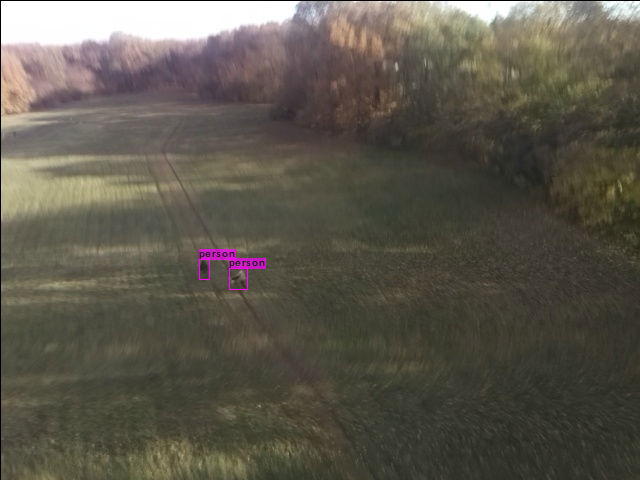
\includegraphics[width=.7\linewidth]{rys03/rozpoznane_yolo.jpg}
	\label{yolo_example}
\end{figure}

\section{Oprogramowanie klienckie}

Aplikacja kliencka pozwala na wykonanie następujących działań:

\begin{itemize}
	\item zaplanowanie przelotu:
	\begin{itemize}
		\item zaplanowanie trasy,
		\item wybór prędkości, z jaką mają być pokonywane konkretne segmenty trasy,
		\item wybór segmentów trasy, podczas których mają być wykonywane zdjęcia,
		\item zaplanowanie godziny wylotu.
	\end{itemize}
	\item podgląd telemetrii w czasie lotu,
	\item przegląd danych teletrycznych zapisanych z poprzednich lotów:
	\begin{itemize}
		\item podlgąd trasy pokonanej przez maszynę,
		\item podgląd wykonanych przez maszynę zdjęć,
				wraz z informacjami o rozpoznanych obiektach,
	\end{itemize} 
\end{itemize}

Najbardziej wymagającym z wymagań jest obsługa mapy, która będzie obecna we wszystkich
widokach aplikacji. W systemie została wykorzystana biblioteka \texttt{Leaflet}, 
służąca do wizualizowania danych na mapach. Biblioteka napisana jest z myślą o technologiach 
webowych, aplikacja kliencka została więc zrealizowana jako aplikacja webowa.
Wykorzystanym w aplikacji frameworkiem \texttt{JavaScript} jest \texttt{VueJS}. 

\begin{figure}[H]
	\centering
	\caption{ Widok aplikacji klienckiej, odpowiedzialny za planowanie tras. }
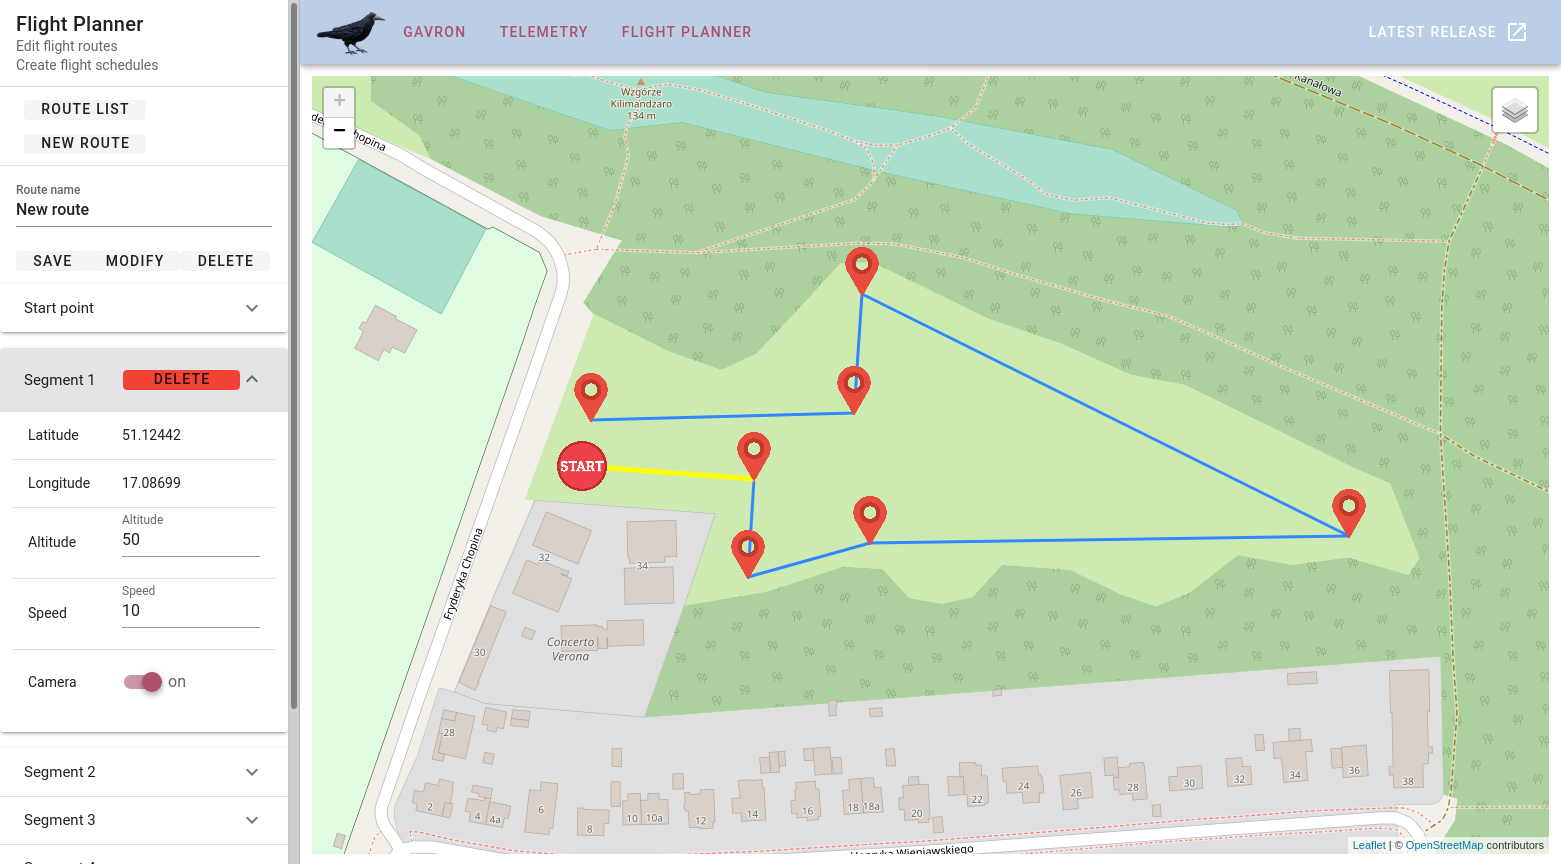
\includegraphics[width=\linewidth]{rys03/flight_planner.png}
	\label{frontend_flight_planner}
\end{figure}


\section{Struktura repozytoriów} \label{repo_structure}

\subsection{Konfiguracja \textit{CI/CD}}

Jak zaznaczono w zakresie pracy (\ref{intro_scope}), system zaopatrzony jest w  
mechanizmy automatyzujące testowanie i wdrażanie nowych 
funkcjonalności. Popularne narzędzia do ciągłej integracji, takie jak
\textit{Jenkins}, \textit{Gitlab CI} czy \textit{Travis CI}, wykorzystują specjalny
plik konfiguracyjny umieszczony w repozytorium. Konfiguracja zawiera zestaw kroków,
dzięki którym kod obecny w repozytorium zostanie automatycznie
zbudowany, przetestowany i wdrożony. Wykorzystywanym w projekcie narzędziem \textit{CI/CD}
jest \textit{Gitlab CI}, ktory oczekuje, że w głównym folderze repozytorium będzie 
znajdował się specjalny plik konfiguracyjny, o nazwie \texttt{gitlab-ci.yml}. 
Jest on obecny we wszystkich repozytoriach projektowych.


\subsection{Wspólne punkty stykowe - \texttt{git submodules}}

Komunikacja pomiędzy komponentami systemu realizowana jest za pośrednictwem
pakietów \texttt{Protobuf}, opisanych w rozdziale \ref{protobuf_chapter}.
Każde z repozytoriów musi więc posiadać pliki, zawierające definicje pakietów,
wygenerowane za pomocą kompilatora \texttt{Protobuf}. 

Możliwe jest utrzymywanie kopii definicji pakietów w każdym projektowym repozytorium,
jednak takie rozwiązanie szybko doprowadzi do konieczności wykonywania dużej ilości
ręcznych poprawek w kodzie, za każdym razem gdy zmieni się standard pakietów. 
Nawet przy niewielkiej liczbie repozytoriów, łatwo tu o błąd programisty. 

Napisanie biblioteki z definicjami pakietów nie jest tutaj odpowiednim rozwiązaniem, 
ponieważ biblioteki pisane są zazwyczaj pod konkretny język programowania. Komponenty
systemu, które przetwarzają telemetrię są napisane w językach \textit{Python} i 
\textit{TypeScript} -- nie jest więc możliwe napisanie dla nich wspólnej biblioteki.

System kontroli wersji \texttt{git} zawiera funkcjonalność
\texttt{git submodules}\cite{git_submodules}, która została wykorzystana
w projekcie do rozwiązania problemu wspólnych definicji pakietów.

Definicje pakietów, wraz z wygenerowanymi implementacjami w wielu językach, utrzymywane 
są w osobnym repozytorium, które pobierane jest jako submoduł dla pozostałych projektów.
Dzięki temu, możliwa jest aktualizacja repozytorium z definicjami pakietów, a następnie
pobranie nowych definicji do wszystkich innych  repozytoriów, które wykorzystują
submoduł z definicjami. 



\section{Architektura systemu - podsumowanie}

\begin{figure}[H]
\centering\small
\caption{
	Architektura systemu - wykorzystane technologie
}
\label{technologies_diagram}
\hspace{-1.2cm}
\begin{forest}
	% forest preamble: determine layout and format of tree
	direction switch, 
	for tree={fork sep=2em, l sep=0.5cm, s sep=0.6cm}
	[ ,yshift=3em,alias=LP, s sep=2.2cm
	  [ \textbf{Dron}
		[ Kontroler lotu 
		  [ \texttt{ArduPilot} ]
		]
		[ Komputer pokładowy, name=flight_computer
		 [ Raspberry Pi ]
		 [ \texttt{Dronekit-Python} ]
		 [ \texttt{pymavlink} ]
		]
	  ]
	  [ \textbf{Serwer webowy}, %yshift=0.5cm
		[ Serwer telemetrii, name=telem_server
			[ \texttt{asyncio } ]
			[ \texttt{UDP} ]
			[ \texttt{WebSocket} ]
		]
		[ Rest API: odczyt i zapis
		  [ \texttt{django} ]
		]
		[ Przesył zdjęć 
		  [ \texttt{imagezmq} ]
		]
		[ Sztuczna inteligencja
		  [ \texttt{yolo} ]
		]
	  ]
	  [ \textbf{Aplikacja kliencka}, xshift=0.1cm
		[ \texttt{VueJS} 
			[ \texttt{Leaflet} ]
			[ \texttt{WebSocket}, name=front_websocket]
		]
	  ]
	]
	\node
		[entity, yshift=-17cm, xshift=4.5cm, align=center](definitions)
		{ Definicje wiadomości \texttt{protobuf} };
	\draw[->] (definitions) to[out=north east, in=south east] node[fill=white,pos=.6]{Submoduł} (telem_server); % leave fill=white away in order to get your image. pos=. is optional. Default would be .5
	\draw[->] (definitions) to[out=north east, in=south east] node[fill=white,pos=.6]{Submoduł} (front_websocket); % leave fill=white away in order to get your image. pos=. is optional. Default would be .5
	\draw[->] (definitions) to[out=west, in=south east] node[fill=white,pos=.6]{Submoduł} (flight_computer); % leave fill=white away in order to get your image. pos=. is optional. Default would be .5
\end{forest}
\end{figure}
